\chapter{编写操作系统内核}

从内存管理,输入输出,多进程,分时四个模块丰富操作系统的内容

\section{内存管理}

内存 (RAM) 是计算机中不可或缺的重要硬件,所有程序的运行都是在内存中进行的,
而CPU访问硬盘数据也必须先经过内存交换才得以实现,内存在加速CPU访问硬盘居功至伟。
由内存的重要性可知内存管理在操作系统中也非常重要。	

内存管理设计的主要目的是快速并且高效的分配内存空间,并在适当的时间释放并回收内存空间。
根据内存管理的设计目的,内存管理的数据结构如下:

\inputminted[tabsize=2, firstline=137, lastline=143,
linenos=true]{c}{../ZOS/src/kernel/bootpack.h}

\begin{description}
\item[frees:]可用信息数目
\item[maxfrees:]用于观察可用状况:frees的最大值
\item[lostsize:]释放失败的内存的大小总和
\item[losts:]释放失败次数
\end{description}

经过内存初始化和释放所有内存空间后,内存管理正常运行。

\subsection{内存分配}

\begin{listing}[H]
  \inputminted[tabsize=2, firstline=68, lastline=80,
  linenos=true]{c}{../ZOS/src/kernel/memory.c}
\end{listing}

\subsection{内存释放}

为保证磁盘空闲空间尽可能不呈现碎片化,内存释放主要分为三种情况:

\begin{description}
\item[前端空闲:]释放内存的相连前端是空闲内存或释放内存相连两端都是空闲内存
\item[后端可用:]释放内存的相连后端是空闲空间
\item[前端后端均不可用:]挪动空闲空间以合并
\end{description}

已知:待释放的空间的开始地址和空间大小

\newpage

前端空闲如图\ref{fig:mem0}和图\ref{fig:mem1}所示: 

\begin{figure}[h]
  \centering
  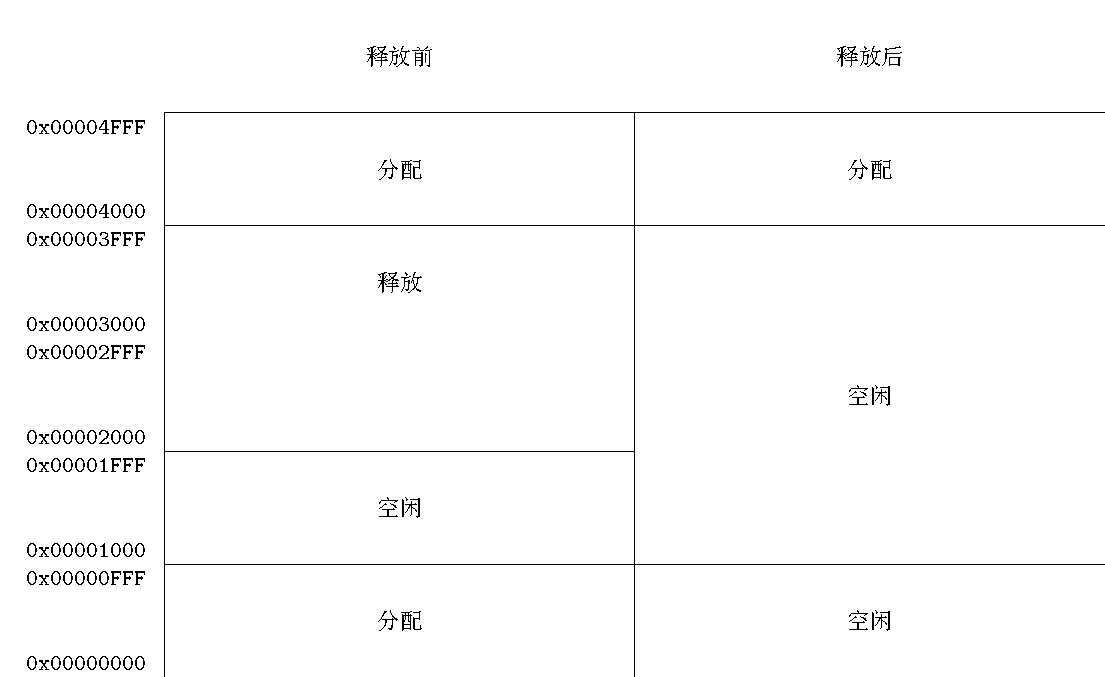
\includegraphics[width=.7\textwidth]{fig/mem0.pdf}
  \caption{前端空闲}
  \label{fig:mem0}
\end{figure}

\begin{figure}[h]
  \centering
  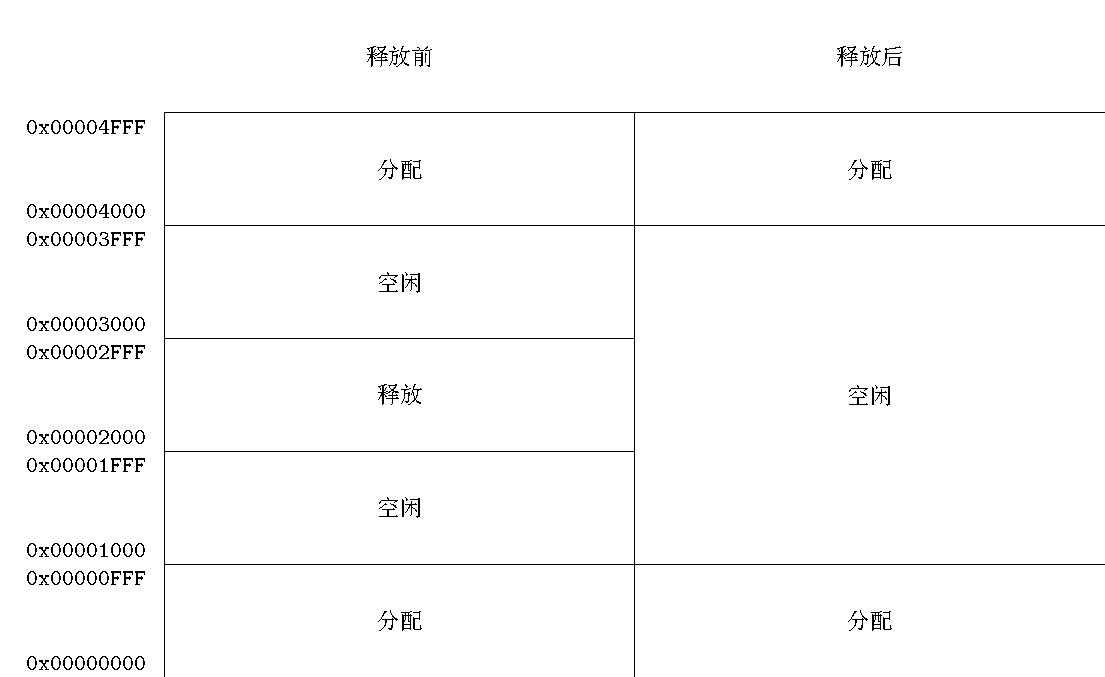
\includegraphics[width=.7\textwidth]{fig/mem1.pdf}
  \caption{前端可用,且后端空闲}
  \label{fig:mem1}
\end{figure}

实现如下:

\begin{listing}[H]
  \inputminted[tabsize=2, firstline=98, lastline=116,
  linenos=true]{c}{../ZOS/src/kernel/memory.c}
\end{listing}

后端空闲:

\begin{figure}[h]
  \centering
  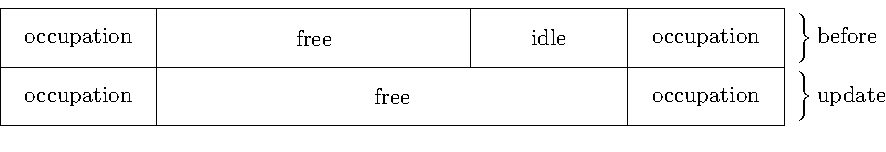
\includegraphics[width=.7\textwidth]{fig/mem2.pdf}
  \caption{后端空闲}
  \label{fig:mem3}
\end{figure}

实现如下:

\begin{listing}[H]
  \inputminted[tabsize=2, firstline=118, lastline=127,
  linenos=true]{c}{../ZOS/src/kernel/memory.c}
\end{listing}

前端后端均被占用:

\begin{figure}[h]
  \centering
  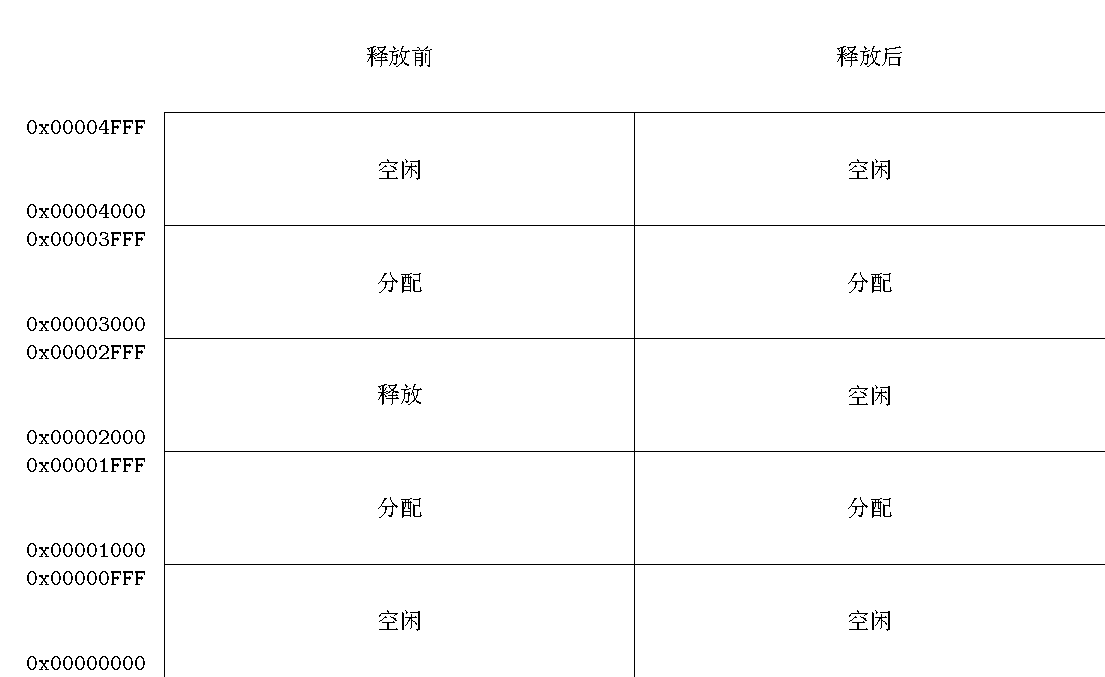
\includegraphics[width=.7\textwidth]{fig/mem3.pdf}
  \caption{前端后端均被占用}
  \label{fig:mem4}
\end{figure}

实现如下:

\begin{listing}[H]
  \inputminted[tabsize=2, firstline=128, lastline=141,
  linenos=true]{c}{../ZOS/src/kernel/memory.c}
\end{listing}

\section{输入输出}

输入作为人与计算机之间最基本的交互方式,其中键盘和鼠标作为标准输入设备。

\subsection{键盘输入}

\begin{listing}[H]
  \inputminted[tabsize=2, firstline=162, lastline=170,
  linenos=true]{c}{../ZOS/src/kernel/bootpack.c}
\end{listing}

\subsection{鼠标输入}

\begin{listing}[H]
  \inputminted[tabsize=2, firstline=247, lastline=265,
  linenos=true]{c}{../ZOS/src/kernel/bootpack.c}
  \inputminted[tabsize=2, firstline=329, lastline=338,
  linenos=true]{c}{../ZOS/src/kernel/bootpack.c}
\end{listing}

\subsection{标准输出}


\section{多道程序系统}

现代的计算机已经不仅仅作为数字计算的工具,而进入大众生活的计算机被赋予了更多的生活需求,
用户可能在看电影的同时查看电子邮件,也有可能在写论文的时候进入浏览器查询相关资料,
但是更重要的是计算机往往在用户不经意间打开防病毒软件等保证用户计算机的安全\cite{tanenbaum2009modern}。

由此可见多进程的工作方式在计算机工作中同样不可或缺。

但是在实际的处理过程中,计算机并不能同时处理多个程序,所以必须采用分时的设计,
关于分时操作系统的设计在下一节。
在此有两个概念,同时处理和多个程序,同时处理属于分时,多道程序属于多道程序设计。

首先要处理的问题是如何在运行多个程序,。

\section{分时操作系统}

在上一节中说到分时是使得在用户看来计算机的多道程序同时运行,多道程序已经实现了,
分时简单说是使得CPU在用户不能明显感觉到的时间间隔内切换运行多个程序,在切换的过程中...
